\documentclass[aspectratio=169]{beamer}
\usetheme{simple}

\input{preamble/preamble.tex}
\input{preamble/preamble_math.tex}
% \input{preamble/preamble_acronyms.tex}

\title{Variational Inference}
\subtitle{STATS 305B: Applied Statistics II}
\author{Scott Linderman}
\date{\today}



\begin{document}

\maketitle


\begin{frame}{Recap}

We've covered several approaches for Bayesian inference...
\begin{itemize}
    \item \textbf{Exact inference:} for simple models (e.g. conjugate exponential family models) where the posterior is available in closed form.
    \item \textbf{Laplace Approximation:} for unimodal posteriors where you can find the mode and local curvature.  
    \item \textbf{Markov Chain Monte Carlo:} for sampling from the posterior when it's difficult to compute or approximate.
    \begin{itemize}
        \item \textbf{Metropolis-Hastings: } a very general MCMC algorithm, and the building block for many other MCMC techniques.
        \item \textbf{Gibbs sampling:} an MCMC algorithm that iteratively samples conditional distributions for one variable at a time. This works well for conditionally conjugate models with weak correlations.
        \item \textbf{Hamiltonian Monte Carlo: } an MCMC algorithm to draw samples from the posterior by leveraging gradients of the log joint probability. This works well for more general posteriors over continuous variables.
    \end{itemize}
\end{itemize}

\end{frame}


\begin{frame}{Outline}

    Today we'll talk about another approach to approximate Bayesian inference called \textbf{variational inference (VI)}.
    
    The key idea is to approximate the posterior with the closest member of a parametric family. 

    Instead of a sampling problem, this is an optimization problem.
    
\end{frame}



\begin{frame}[t]{Why Variational Inference?}

    % We liked the Laplace approximation because they were deterministic and often very efficient to compute, but they were biased for non-Gaussian posteriors.
    
    MCMC methods are asymptotically unbiased (though for finite samples there is a transient bias that shrinks as $O(M^{-1})$). The real issue is variance: it only shrinks as $O(M^{-1/2})$.
    
    \textbf{Motivation: } With finite computation, can we get better posterior estimates by trading asymptotic bias for smaller variance? 
    
    \textbf{Idea: } approximate the posterior by with a simple, parametric form (though not strictly a Gaussian on the mode!). Optimize to find the approximation that is as ``close'' as possible to the posterior.
        
\end{frame}
    
\begin{frame}{Notation}
    This notation could be a bit confusing. Let,
    \begin{itemize}
        \item $\mbtheta \in \reals^D$ denote \textbf{all of latent variables and parameters} we wish to infer. 

        \item $p(\mbtheta \mid \mbx)$ denote the true posterior distribution we want to approximate.
        
        \item $q(\mbtheta; \mblambda)$ denote a parametric \textit{variational approximation} to the posterior where...
        
        \item $\mblambda$ denotes the \textit{variational parameters} that we will optimize.
        
        \item $D(q \, \| \, p)$ denote a \textit{divergence measure} that takes in two distributions $q$ and $p$ and returns a measure of how similar they are.
    \end{itemize}
\end{frame}
    
\begin{frame}{A view of variational inference}
    \centering
    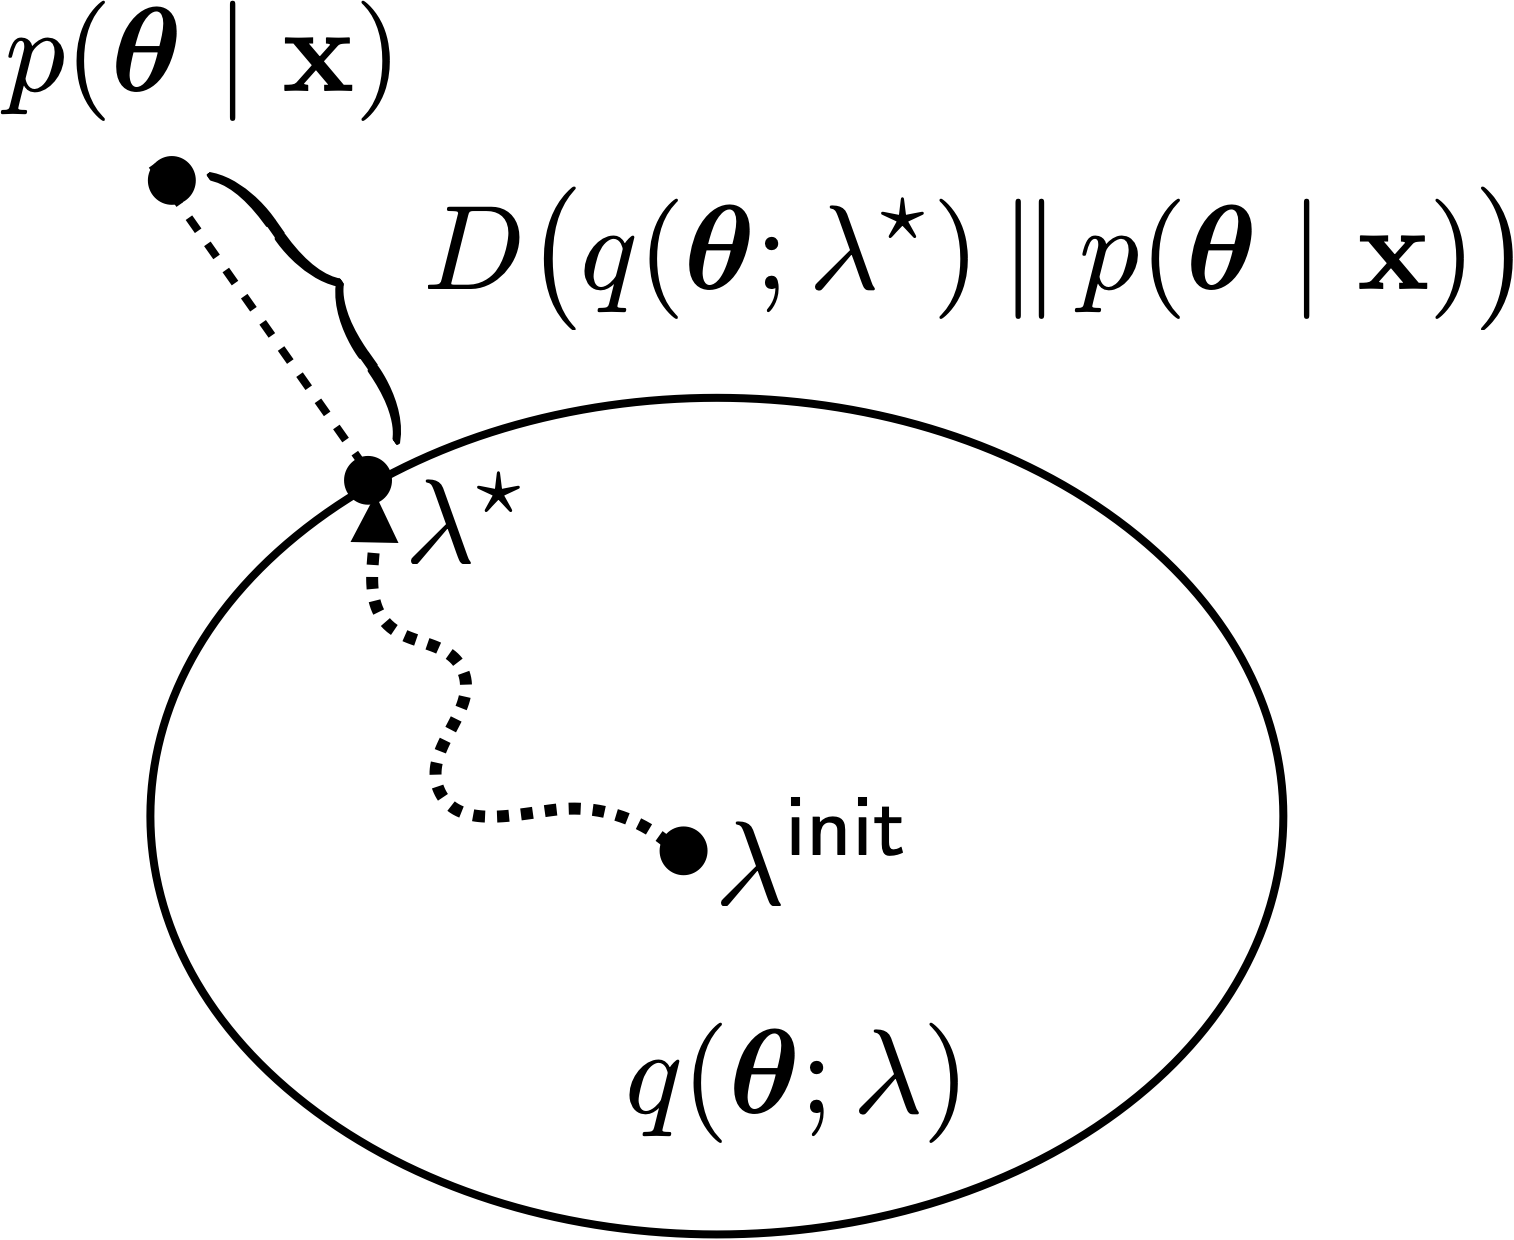
\includegraphics[width=.5\textwidth]{09_vi/vi.png}
\end{frame}

\begin{frame}{Three key questions}
    \begin{itemize}
        \item \textit{What parametric family should we use? }
        \item \textit{How should we measure closeness? }
        \item \textit{How do we find the closest distribution in that family?}        
    \end{itemize}
    
\end{frame}
    

\begin{frame}{Coordinate Ascent Variational Inference (CAVI)}
\begin{itemize}
    \item \textit{What parametric family should we use? }
    \begin{itemize}
        \item The \textbf{mean-field family}.
    \end{itemize}
    
    \item \textit{How should we measure closeness? }
    \begin{itemize}
        \item The \textbf{Kullback-Leibler (KL)} divergence.
    \end{itemize}
    
    \item \textit{How do we find the closest distribution in that family?}
    \begin{itemize}
        \item \textbf{Coordinate ascent}, assuming we have a conditionally conjugate model.
    \end{itemize}
\end{itemize}

\end{frame}

\begin{frame}{Gradient-based Variational Inference}

\begin{itemize}
    \item \textit{What parametric family should we use? }
    \begin{itemize}
        \item Pretty much any $q$, as long as we can sample from it and evaluate the log density.
    \end{itemize}
    
    \item \textit{How should we measure closeness? }
    \begin{itemize}
        \item The \textbf{Kullback-Leibler (KL)} divergence.
    \end{itemize}
    
    \item \textit{How do we find the closest distribution in that family?}
    \begin{itemize}
        \item \textbf{Stochastic gradient ascent} using Monte Carlo estimates of the ELBO and its gradient.
    \end{itemize}
\end{itemize}

Gradient-based VI methods go under a few different names: black-box VI (BBVI), automatic differentiation VI (ADVI), fixed-form VI...

\end{frame}
    
    
% \begin{frame}{The mean-field family}
%     The \textit{mean-field family} gets its name from statistical mechanics. It treats each latent variable and parameter as independent with its own variational parameter,
%     \begin{align*}
%         q(\mbtheta; \mblambda) &= \prod_{j=1}^J q(\theta_d; \lambda_d).
%     \end{align*}
    
%     For example, in the GMM, the mean field approximation treats the cluster proportions, means, and assignments as independent,
%     \begin{align*}
%         q(\mbtheta; \mblambda) &= 
%         q(\mbpi; \widetilde{\mbalpha}) 
%         \prod_{k=1}^K q(\mbmu_k; \widetilde{\nu}_k, \widetilde{\mbphi}_k) 
%         \prod_{n=1}^N q(z_{n}; \widetilde{\mbomega}_n)
%     \end{align*}
%     for some functional forms and parameterizations that we will specify shortly.
    
%     \textbf{Question: } Does the true posterior factor in this way? If not, why not?
    
% \end{frame}
    
\begin{frame}{The Kullback-Leibler (KL) divergence}
    The KL divergence is a measure of closeness between two distributions. It is defined as,
    \begin{align*}
        \KL{q(\mbtheta; \mblambda)}{p(\mbtheta \mid \mbx} &= \E_{q(\mbtheta; \mblambda)} \left[ \log \frac{q(\mbtheta; \mblambda)}{p(\mbtheta \mid \mbx)} \right] \\
        &= \E_{q(\mbtheta; \mblambda)} \left[ \log q(\mbtheta; \mblambda) \right] 
        - \E_{q(\mbtheta; \mblambda)} \left[ \log p(\mbtheta \mid \mbx) \right] 
        % \\
        % &= \underbrace{\bbH[q(\mbtheta; \mblambda), p(\mbtheta \mid \mbx)]}_{\text{cross entropy}} - \underbrace{\bbH[q(\mbtheta; \mblambda)]}_{\text{entropy}}
    \end{align*}
    
    It has some nice properties:
    \begin{itemize}
        \item It is non-negative.
        
        \item It is zero iff $q(\mbtheta; \mblambda) \equiv p(\mbtheta \mid \mbx)$.
        
        \item It is defined in terms of expectations wrt $q$.
    \end{itemize}
    
    But it's also a bit weird... 
    \begin{itemize}
        \item It's asymmetric ($\KL{q}{p} \neq \KL{p}{q}$).
    \end{itemize}
\end{frame}
    
\begin{frame}{The evidence lower bound (ELBO) from another angle}
        More concerning, the KL divergence involves the posterior $p(\mbtheta \mid \mbx)$, which we cannot compute!
        
        But notice that...
        \begin{align*}
            \KL{q(\mbtheta; \mblambda)}{p(\mbtheta \mid \mbx}
            &= \E_{q(\mbtheta; \mblambda)} \left[ \log q(\mbtheta; \mblambda) \right] 
            - \E_{q(\mbtheta; \mblambda)} \left[ \log p(\mbtheta \mid \mbx) \right] \\
            &= \E_{q(\mbtheta; \mblambda)} \left[ \log q(\mbtheta; \mblambda) \right] 
            - \E_{q(\mbtheta; \mblambda)} \left[ \log p(\mbtheta, \mbx) \right] 
            + \E_{q(\mbtheta; \mblambda)}\left[ \log p(\mbx)\right] \\
            &= \underbrace{\E_{q(\mbtheta; \mblambda)} \left[ \log q(\mbtheta; \mblambda) \right] 
            - \E_{q(\mbtheta; \mblambda)} \left[ \log p(\mbtheta, \mbx) \right]}_{\text{negative ELBO}, -\cL(\mblambda)}
            + \underbrace{\log p(\mbx)}_{\text{evidence}}
        \end{align*}
    The first term involves the log joint, which we can compute, and the last term is independent of the variational parameters! 
    
    Rearranging, we see that $\cL(\mblambda)$ is a lower bound on the marginal likelihood, aka the evidence,
    \begin{align*}
        \cL(\mblambda) &= \log p(\mbx) - \KL{q(\mbtheta; \mblambda)}{p(\mbtheta \mid \mbx} 
        \leq \log p(\mbx).
    \end{align*}
    That's why we call it the \textbf{evidence lower bound (ELBO)}.
\end{frame}
    
\begin{frame}{Viewer discretion advised...}
    
    \centering
    % \includemedia[
    %     width=0.75\linewidth,height=0.3375\linewidth, % 16:9
    %     activate=pageopen,
    %     flashvars={
    %     modestbranding=1 % no YT logo in control bar
    %     &autohide=1 % controlbar autohide
    %     &showinfo=0 % no title and other info before start
    %     &rel=0 % no related videos after end
    %     }
    %     ]{}{https://www.youtube.com/watch?v=jugUBL4rEIM}
    \url{https://www.youtube.com/watch?v=jugUBL4rEIM}
    
\end{frame}


\begin{frame}[t]{Setup}
    % Let $\mbtheta$ denote parameters to be inferred and $p(\mbtheta \mid \mbX)$ the true posterior to be approximated.
    
    % Let $\cQ = \{q(\mbtheta; \mblambda): \mblambda \in \mbLambda\}$ denote the variational family --- a parametric family of distributions indexed by $\mblambda$ that we will optimize over in variational inference. 
    
    The optimal approximation is,
    \begin{align*}
        q^\star(\mbtheta; \mblambda) 
        &= \argmin_{q \in \cQ} \KL{q(\mbtheta; \mblambda)}{p(\mbtheta \mid \mbX)}
    \end{align*}
    or equivalently
    \begin{align*}
        \mblambda^\star
        &= \argmin_{\mblambda \in \mbLambda} \KL{q(\mbtheta; \mblambda)}{p(\mbtheta \mid \mbX)} \\
        &= \argmax_{\mblambda \in \mbLambda} \cL(\mblambda)
    \end{align*}
    where $\cL(\mblambda)$ denotes the \textbf{evidence lower bound (ELBO)},
    \begin{align*}
        \cL(\mblambda) &= \E_{q(\mbtheta; \mblambda)} \left[\log p(\mbX, \mbtheta) - \log q(\mbtheta; \mblambda) \right]
    \end{align*}
\end{frame}
    
\begin{frame}{Optimizing the ELBO with coordinate ascent}
    We want to find the variational parameters $\mblambda$ that minimize the KL divergence or, equivalently, maximize the ELBO.
    
    For the mean-field family, we can typically do this via \textbf{coordinate ascent}. 
    
    Consider optimizing the parameters for one factor~$q(\theta_d; \lambda_d)$. As a function of $\lambda_d$, the ELBO is,
    \begin{align*}
        \cL(\mblambda) 
        &= 
        \E_{q(\theta_d; \lambda_d)}\left[ \E_{q(\mbtheta_{\neg d}; \mblambda_{\neg d})} \left[ \log p(\mbtheta, \mbx) \right] \right] -
        \E_{q(\theta_d; \lambda_d)}[\log q(\theta_d; \lambda_d)] + c \\
        &= 
        \E_{q(\theta_d; \lambda_d)}\left[ \E_{q(\mbtheta_{\neg d}; \mblambda_{\neg d})} \left[ \log p(\theta_d \mid \mbtheta_{\neg_d}, \mbx) \right] \right] -
        \E_{q(\theta_d; \lambda_d)}[\log q(\theta_d; \lambda_d)] + c' \\
        &= -\KL{q(\theta_d; \lambda_d)}{\tilde{p}(\theta_d)} + c''
    \end{align*}
    where 
    \begin{align*}
        \label{eq:cavi_form}
        \tilde{p}(\theta_d) &\propto
        \exp \left\{ \E_{q(\mbtheta_{\neg d}; \mblambda_{\neg d})} \left[ \log p(\theta_d \mid \mbtheta_{\neg d}, \mbx) \right] \right\}
    \end{align*}
    The ELBO is maximized wrt $\lambda_d$ when this KL is minimized; i.e. when $q(\theta_d ; \lambda_d) = \tilde{p}(\theta_d)$, the exponentiated expected log conditional probability, holding all other factors fixed.
\end{frame}




% \begin{frame}[t]{Generic M-step with gradient ascent}
%     For exponential family mixture models and simple factor analysis, the M-steps had closed form.
    
%     For deep generative models, however, we need a more general approach.
    
%     If the parameters are unconstrained and the ELBO is differentiable wrt $\mbtheta$, we can use \textbf{gradient ascent}. 
    
%     Repeat:
%     \begin{align*}
%         \mbtheta &\leftarrow \mbtheta + \alpha \nabla_{\mbtheta} \cL(q, \mbtheta) 
%         = \mbtheta + \alpha \sum_{n=1}^N \mathbb{E}_{q(\mbtheta)} \left[ \nabla_{\mbtheta} \log p(\mbx, \mbtheta; \mbtheta) \right]
%     \end{align*}
%     with \textbf{step size} $\alpha$. Typically, you decrease the step size over iterations so that~$\alpha_1 \geq \alpha_2 \geq \ldots$
% \end{frame}

\begin{frame}[t]{Optimizing the ELBO with stochastic gradient ascent}
    \begin{itemize}
    \item<1-> \textbf{Idea: } Assume the variational parameters $\mbLambda$ are unconstrained (i.e., $\mbLambda = \mathbb{R}^Q$), then perform (stochastic) gradient ascent. 
    
    \item<2-> If the parameters are unconstrained and the ELBO is differentiable, we can use \textbf{gradient ascent}. 
    Repeat:
    \begin{align*}
        \mblambda &\leftarrow \mblambda + \alpha \nabla_{\mblambda} \cL(\mblambda) 
    \end{align*}
    with \textbf{step size} $\alpha$. Typically, you decrease the step size over iterations so that~$\alpha_1 \geq \alpha_2 \geq \ldots$
    
    \item<3-> More generally, we can use \textbf{\textit{stochastic} gradient ascent} with an estimate of the gradient, $\widehat{\nabla}_{\mblambda} \cL(\mblambda)$, as long as it is unbiased,
    \begin{align*}
        \E[\widehat{\nabla}_{\mblambda} \cL(\mblambda)] = \nabla_{\mblambda} \cL(\mblambda).
    \end{align*}
    \end{itemize}
\end{frame}

\begin{frame}[t]{Monte Carlo gradient estimation}
No problem! We'll just use ordinary Monte Carlo to estimate the gradient. But we run into a problem...
\begin{align*}
\nabla_{\mblambda} \cL(\mblambda) 
&= \nabla_{\mblambda} \E_{q(\mbtheta; \mblambda)} \left[ \log p(\mbx, \mbtheta) - \log q(\mbtheta; \mblambda) \right] \\
&\textcolor{red}{\neq} \;  \E_{q(\mbtheta; \mblambda)} \left[ \nabla_{\mblambda} \left(\log p(\mbx, \mbtheta) - \log q(\mbtheta; \mblambda)\right) \right].
\end{align*}

\textbf{Problem: } Why can't we simply bring the gradient inside the expectation?
\end{frame}

\begin{frame}[t, allowframebreaks]{The ``score function'' gradient estimator}
    The basic problem is that the variational parameters $\mblambda$ determine the distribution we are taking an expectation under.  However, there are a few ways to obtain unbiased estimates of the gradient.
    
    One approach is called the \textbf{score function gradient estimator} or the \textbf{REINFORCE estimator}~\citep{williams1992simple}. It is based on the following identity,
    
    \begin{align*}
        \nabla_{\mblambda} \log q(\mbtheta; \mblambda) &= \frac{\nabla_{\mblambda} q(\mbtheta; \mblambda)}{q(\mbtheta; \mblambda)}
    \end{align*}
    where the l.h.s. is called the score function of distribution $q$.
    
    We can use this identity to obtain an unbiased estimate of the gradient of an expectation,
    \begin{align*}
        \nabla_{\mblambda} \E_{q(\mbtheta; \mblambda)} \left[ h(\mbtheta) \right] 
        &= \nabla_{\mblambda} \int q(\mbtheta; \mblambda) \, h(\mbtheta) \dif \mbtheta \\
        &= \int \left(\nabla_{\mblambda} q(\mbtheta; \mblambda)\right) h(\mbtheta) \dif \mbtheta \\
        &= \int \left(q(\mbtheta; \mblambda) \nabla_{\mblambda} \log q(\mbtheta; \mblambda)\right) h(\mbtheta)  \dif \mbtheta \\
        &= \E_{q(\mbtheta; \mblambda)} \left[ \left(\nabla_{\mblambda} \log q(\mbtheta; \mblambda)\right) h(\mbtheta) \right]
    \end{align*}
    From this identity, we can obtain an unbiased Monte Carlo estimate,
    \begin{align*}
        \widehat{\nabla}_{\mblambda} \E_{q(\mbtheta; \mblambda)}[h(\mbtheta)] &= \frac{1}{M} \sum_{m=1}^M \left[ \nabla_{\mblambda} \log q(\mbtheta^{(m)}; \mblambda) \, h(\mbtheta^{(m)}) \right]; 
        \qquad \mbtheta^{(m)} \iid{\sim} q(\mbtheta; \mblambda)
    \end{align*}
    
    \textbf{Notes:}
    \begin{enumerate}
        \item The exchange of the gradient and the integral is allowed as long as the dominated convergence theorem holds, and it usually does for ML applications.
        
        \item The score function gradient estimator is broadly applicable; e.g. it works for discrete and continuous latent variables~$\mbtheta$. We just need the log density to be continuously differentiable wrt $\mblambda$ and to be able to sample from~$q$. 
        
        \item If $h$ is a function of both $\mbtheta$ and $\mblambda$, you need to apply the product rule. This gives another term,
        \begin{align*}
        \nabla_{\mblambda} \E_{q(\mbtheta; \mblambda)} \left[ h(\mbtheta, \mblambda) \right] 
        &= \E_{q(\mbtheta; \mblambda)} \left[ \left(\nabla_{\mblambda} \log q(\mbtheta; \mblambda)\right) h(\mbtheta, \mblambda) \right]
        + \E_{q(\mbtheta; \mblambda)} \left[ \nabla_{\mblambda} h(\mbtheta, \mblambda) \right]
        \end{align*}
        
    \end{enumerate}
\end{frame}

\begin{frame}[t]{Control variates}
    Though broadly applicable, the score function estimator is often too high variance to be useful. This problem can often be mitigated with \textbf{control variates}. 
    
    Recall that the expectation of the score is zero,
    \begin{align*}
        \E_{q(\mbtheta; \mblambda)} \left[ \nabla_{\mblambda} \log q(\mbtheta; \mblambda)\right] 
        &= \int q(\mbtheta; \mblambda) \nabla_{\mblambda} \log q(\mbtheta; \mblambda) \dif \mbtheta \\
        &= \int \nabla_{\mblambda} q(\mbtheta; \mblambda) \dif \mbtheta \\
        &= \nabla_{\mblambda} \int q(\mbtheta; \mblambda) \dif \mbtheta \\
        &= \nabla_{\mblambda} 1 = 0.
    \end{align*}
    Thus, we can subtract off any \textbf{baseline} from the function of interest without changing the expectation, but potentially reducing variance substantially,
    \begin{align*}
        \E_{q(\mbtheta; \mblambda)} \left[ h(\mbtheta)  \nabla_{\mblambda} \log q(\mbtheta; \mblambda)\right] 
        &= \E_{q(\mbtheta; \mblambda)} \left[ (h(\mbtheta) - b)  \nabla_{\mblambda} \log q(\mbtheta; \mblambda)\right].
    \end{align*}
\end{frame}

\begin{frame}[t]{The pathwise gradient estimator}
\begin{itemize}
    \item<1-> The pathwise gradient estimator has more requirements, but often performs better. Suppose $q(\mbtheta; \mblambda) = \cN(\mbtheta; \mbmu, \diag(\mbsigma^2))$, where $\mblambda = (\mbmu, \log \mbsigma^2)$ are the (unconstrained) variational parameters. Then,
    \begin{align*}
        \mbtheta \sim q(\mbtheta; \mblambda) \quad \iff \quad
        \mbtheta &= r(\mblambda, \mbepsilon), \quad \mbepsilon \sim \cN(\mbzero, \mbI) 
    \end{align*}
    where $r(\mblambda, \mbepsilon) = \mbmu + \mbsigma \mbepsilon$ is a \textbf{reparameterization} of $\mbtheta$ in terms of parameters~$\mblambda$ and ``noise''~$\mbepsilon$.

    \item<2-> We can use the \textbf{law of the unconscious statistician} to rewrite the expectations as,
    \begin{align*}
        \E_{q(\mbtheta; \mblambda)} \left[h(\mbtheta, \mblambda) \right]
        &= \E_{\mbepsilon \sim \cN(\mbzero, \mbI)} \left[h(r(\mblambda, \mbepsilon), \mblambda) \right]
    \end{align*}
    The distribution that the expectation is taken under no longer depends on the parameters $\mblambda$, so we can simply take the gradient inside the expectation,
    \begin{align*}
        \nabla_{\mblambda} \E_{q(\mbtheta; \mblambda)} \left[h(\mbtheta, \mblambda) \right]
        &=  \E_{\mbepsilon \sim \cN(\mbzero, \mbI)} \left[\nabla_{\mblambda} h(r(\mblambda, \mbepsilon), \mblambda) \right]
    \end{align*}

    \item<3->Now we can \textbf{use Monte Carlo to obtain an unbiased estimate of the final expectation.}
    \begin{align*}
        \widehat{\nabla}_{\mblambda} \E_{q(\mbtheta; \mblambda)} \left[h(\mbtheta, \mblambda) \right]
        &= \frac{1}{M} \sum_{m=1}^M \nabla_{\mblambda} h(r(\mblambda, \mbepsilon_m), \mblambda); & \epsilon_m \iid{\sim} \cN(\mbzero, \mbI)
    \end{align*}
    
\end{itemize}
\end{frame}


\begin{frame}[t]{Exercises}
    
\textbf{Exercise:} Come up with a reparameterization of an exponential distribution, $q(\theta; \lambda) = \mathrm{Exp}(\theta; \lambda)$ 

\vspace{4em}

\textbf{Question:} Can you use the pathwise gradient estimator for a Bernoulli posterior, $q(\theta; \lambda) = \mathrm{Bern}(\theta; \lambda)$? 
\end{frame}

\begin{frame}[t]{Empirically comparing estimator variances}
    \begin{figure}
        \centering
        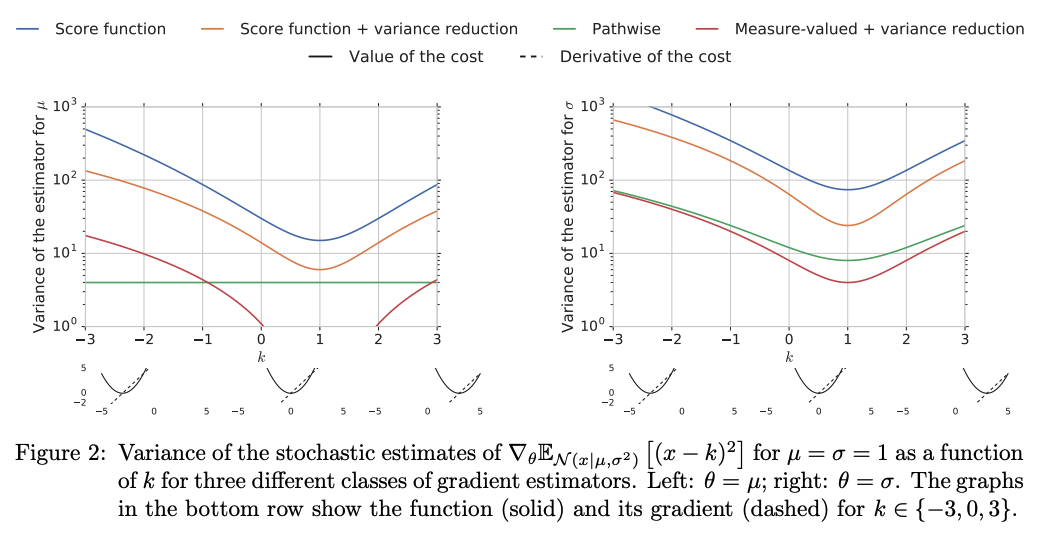
\includegraphics[width=.9\linewidth]{09_vi/mc_gradient.png}
    \end{figure}
    Empirical comparisons from~\citet{mohamed2020monte}.
\end{frame}

\begin{frame}{Working with mini-batches of data}
Often, the ELBO involves a sum over data points,
\begin{align*}
    \cL(\mblambda) &= \E_q [\log p(\mbX, \mbtheta) - \log q(\mbtheta; \mblambda] \\
    &= \E_{q(\mbtheta; \mblambda)} \left[\sum_{n=1}^N \log p(\mbx_n \mid \mbtheta) + \log p(\mbtheta) - \log q(\mbtheta; \mblambda) \right]
    \\
    &= \sum_{n=1}^N \E_{q(\mbtheta; \mblambda)}[\log p(\mbx_n \mid \mbtheta)] - \KL{q(\mbtheta; \mblambda)}{p(\mbtheta)}
\end{align*}

We can view the sum as an ``expectation'' over data indices,
\begin{align*}
    \sum_{n=1}^N \E_{q(\mbtheta; \mblambda)}[\log p(\mbx_n \mid \mbtheta)] &= N \, \E_{n \sim \distUniform(1,N)}[\E_{q(\mbtheta; \mblambda)}[\log p(\mbx_n \mid \mbtheta)]],
\end{align*}
and we can use Monte Carlo to approximate both expectations! (The same is true for Monte Carlo estimators of the gradient of the ELBO.)
\end{frame}

\begin{frame}[t]{SGD convergence and extensions}
    When does SGD work? This is a well studied problem in stochastic optimization~\citep{bottou1998online, robbins1971convergence}.
    
    Under relatively mild conditions, SGD converges to a \textbf{local minimum} if the step sizes obey the \textbf{Robbins-Monro condtions},
    \begin{align*}
        \sum_{i=0}^\infty \alpha_i &= \infty \qquad \text{and} \qquad
        \sum_{i=0}^\infty \alpha_i^2 < \infty
    \end{align*}
    
    There have been dozens of extensions to basic SGD including,
    \begin{itemize}
        \item SGD with momentum
        \item AdaGrad \citep{duchi2011adaptive}
        \item RMSProp 
        \item Adam \citep{kingma2014adam}
    \end{itemize}
\end{frame}



\begin{frame}[t,allowframebreaks]
        \frametitle{References}
        \bibliographystyle{unsrtnat}
        \bibliography{refs.bib}
\end{frame}

\end{document}